\section{复杂的论证性语段}

\begin{logicbox}[title=引言]
\textit{复杂的论证性语段是我们在实践中常见的推理形式,它们涉及多个前提和结论的交织,通过掌握分析方法,我们能更清晰地理解和评估这些论证。}
\end{logicbox}

实际论证有可能是非常复杂的。有些语段中的论证是由几个论证多重复合而成,语段中有些命题只作为前提,有些命题既作为前提又作为\textbf{分结论},这样的语段分析起来就比较困难。\textbf{图示法}的技术就非常有助于分析这种语段,但并不存在一种建构图示以精确地描述这样的语段的机械方法。此外,因为对这种语段可以作几种合理的解释,因此也可以合理地考虑几种不同图示来展现其逻辑结构。

\subsection{复杂语段分析方法}

为了清楚地分析复杂语段,我们必须努力理解作者推理的流程,辨识语段中每个成分的作用。下面的例子(为便于分析,其中的分支命题用数字标出)显示了我们阐明前提和结论之间的联系的方法。一旦辨识出一段话语中所含的论证以及论证之间的关系,我们就能够对这些论证的结论是否真正是从被断定的前提中推论出来的做出判定。

在下列论证集合中,语段最后的结论就是第一个陈述,这不奇怪。有四个前提直接支持这个结论,其中的两个前提又是分结论,逐次得到语段中所断言的其他前提不同方式的支持:

\begin{displayquote}
(1)看来, 用动物实验进行科学研究的做法并不是不必要的或靠不住的; (2)在使用脊椎动物进行实验之前, 实验的草案必须经过包括一名兽医和一名公众代表在内的公共机构委员会进行的再审查, 并且(3)在研究期间, 动物的医疗和卫生情况得到定期监测。(4)研究者需要健康的动物进行科学研究和医学研究, 因为(5)不健康的动物可能导致错误的研究结果。这激励(6)科学家确保他们使用的任何动物健康并且营养良好。此外, (7)用动物进行研究是昂贵的, 因为(8)料学研究的资金受到限制, (9)只有高质量的研究才能通过有力的竞争获得对研究的支持。$^{[49]}$
\end{displayquote}

下面的图示展示了这段话的逻辑结构。检查这样的图示,从那些在图中最高处因而在逻辑串联中也是最早的地方开始,通过用数字替换表达出来的命题,有助于对它们进行"解读"。也就是说,人们能够从推理的几条路线的每一条路径推出最后的结论。

\begin{center}
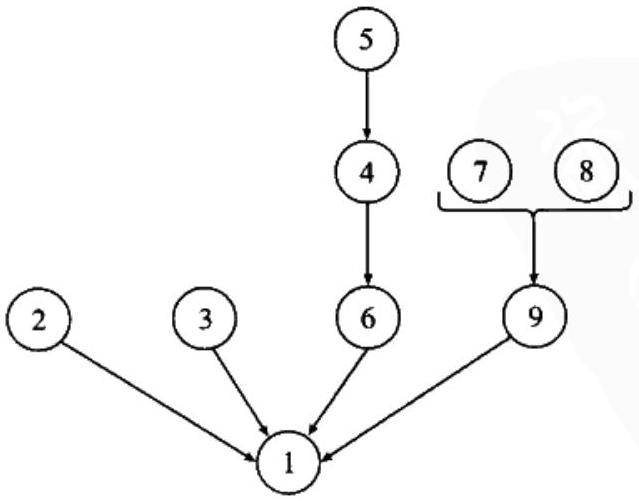
\includegraphics[width=\textwidth]{images/2025_05_15_6a28331d5e7c993ad07ag-072.jpg}
\end{center}

\subsection{处理重复和强调的命题}

在一个论证中,单个的命题有时以不同语词表达的语句形式重复出现,有时是为了强调,有时又被省略。这种强调使得分析工作复杂化。图示法有助于分析,因为我们可以用相同的数字表示相同命题的不同表述。下面一段话由三个清楚的论证构成,有些命题重复多次出现:

\begin{displayquote}
(1)宇宙大爆炸理论正在瓦解……(2)根据正统知识, 宇宙起源于大爆炸——200 亿年前的一次巨大的、非常匀称的爆炸。问题是(3)天文学家通过进一步观测证实: 现存的巨大星系团因为体积太大, 完全不可能在仅仅 200 亿年时间中形成……通过人造卫星所收集的新材料的研究, 以及较早前的地面测量表明(4)星系聚集成绵延数十亿光年的巨大带状, 并且(5)星系之间有亿方光年的距离。因为(6)据观测, 星系移动的速度远不及光速, 数学家证明(7)聚集成这么大的物质团必须要经过至少 1000 亿年时间——是假设的大爆炸时间的五倍……(3)像那么大的一种结构现在看来不可能在 200亿年时间中形成……(2)大爆炸理论认为, 物质均匀地散布在宇宙中。而与这种理想理论相反, (3)这么巨大的星丛无法这么快地形成。$^{[50]}$
\end{displayquote}

在这段话中,报告观察证据的前提(4)、(5)、(6)为(7)即自大爆炸起必须经过非常长的时间提供理由。这被用来支持分结论(以三种略有不同的方式表述)即(3)像那么大的一种结构现在看来因为太大,不可能在那段时间中形成。从 (3)这个结论,结合(2)即对大爆炸理论假设的原始对称和扩散的简短陈述(以两种略有不同的方式表述),我们可以推论出这段话最后的结论(1):大爆炸理论正在瓦解——这段话开头的命题。下面的图示展示了这段话的逻辑关系集:

\begin{center}
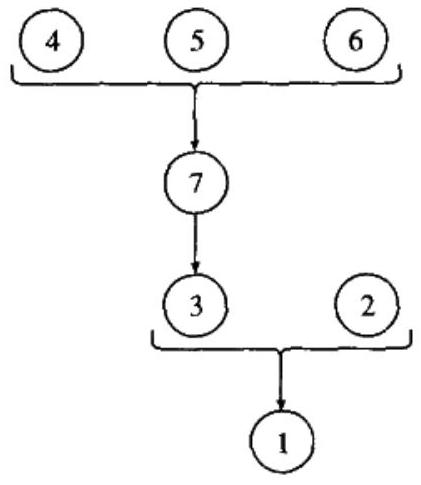
\includegraphics[width=\textwidth]{images/2025_05_15_6a28331d5e7c993ad07ag-073.jpg}
\end{center}

\subsection{处理浓缩的前提}

分析论证,必须注意前提可能以\textbf{浓缩形式}出现的情形,有时前提只以一个名词性短语来表示。在下面的论证中短语"在大气中的散射"作为前提(4),可以重塑为"太阳的能量散射在大气中"。浓缩与重复使得对下列论证的分析更加困难:

\begin{displayquote}
(1)太阳能汽车只是一种试验性的装置, 其他什么都不是。(2)太阳的能量太弱以至于不能发动甚至是日常使用的迷你汽车。(3)进入大气层的太阳能量大约为每平方码 1 千瓦。因为(4)在大气中的散射, 又因为(5)地球上的任何地方一天中平均只有半天时间受到阳光的照射, (6)每天接收的太阳功率平均为 $1 / 6$ 千瓦时到 4千瓦时 $\cdots \cdots$ 对通常规格的汽车的检测表明, (7)若使一辆电车勉强能够工作, 其电池组需要 300 千瓦时的能量。因此, (8)充满汽车电池必须有 40 平方码的原电池, 大约是一辆拖拉机的拖车顶部的尺寸。(1)除了用于昂贵的试验汽车外, 太阳能没有指望成为任何汽车的动力, 太阳能汽车不是一项待开发的技术。这就是结论。$^{[51]}$
\end{displayquote}

这段话中的第一个命题,即"太阳能汽车只是一种试验性的装置,其他什么都不是"的断定,是最后的结论。语段的最后以更加复杂的形式重复了这一结论。这段话的图示为:

\begin{center}
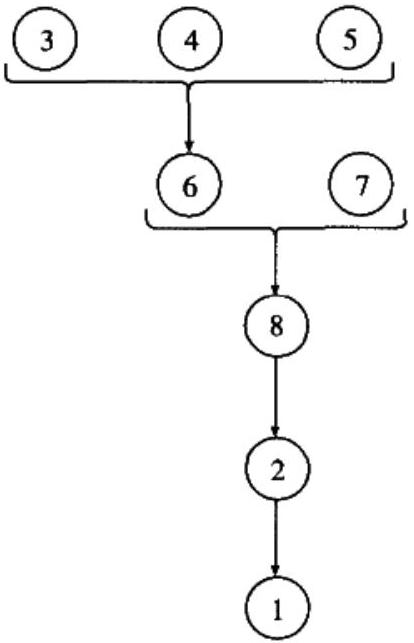
\includegraphics[width=\textwidth]{images/2025_05_15_6a28331d5e7c993ad07ag-074.jpg}
\end{center}

\subsection{融贯的复杂论证分析}

在我们分析复杂的论证性话语时,即使是一些包含许多前提和分结论的语段,我们也经常发现它们是非常融贯的、清楚的。请看一位女编辑为其引起争论的编辑方针进行辩护时所写的一段话:

\begin{displayquote}
本刊(《新英格兰医学杂志》)的主张是(1)不发表不道德的研究报告,忽略它们的料学价值……

我们的主张有三个理由。首先,(2)如果普遍坚持这个主张,只发表合乎道德的研究文章,将会阻止不合乎道德的研究工作的开展。(3)文章的发表是医学研究奖赏制度的一个重要部分。(4)如果研究者知道他们不合乎道德的研究成果不能发表,他们就不会去做不道德的研究。(5)而相反的做法将有助于导致更多的不道德研究工作的开展,因为,如我已表明的,(6)这样的研究可能比较容易开展,因而(7)可能使从事不道德研究工作的人处于有利的竞争地位。其次,(8)即使发表不道德的研究成果不妨碍发表合乎道德的研究成果,为了坚持把合乎道德放在研究第一位的原则,也应该拒绝不道德的研究。(9)如果允许有所松动,我们将逐渐变得习惯于发表不道德的研究成果,并且(10)这将导致对发表合乎道德的研究成果的极大妨碍。最后,(11)对不道德研究成果的拒绝,有利于使社会普遍注意到,甚至某些科学家也不懂得科学研究应是文明的基本尺度。(12)知识尽管很重要,但对一个公平公正的社会来说知识或许远不及得到知识的方法重要。$^{[52]}$
\end{displayquote}

最后的结论也出现在语段开头,(2)、(8)和(11)三个主要命题直接支持这个结论,这三个前提本身又得到处于不同位置的其他几个前提的支持。语段中的众多命题,在导出结论的过程中都有一个清楚的逻辑作用,共同服务于整个语段要证明的结论:不合乎道德的研究报告将不能在《新英格兰医学杂志》上发表,它们的科学价值也应被忽略。下面的图示展示了这个虽然复杂但推理缜密的语段的逻辑结构。

\begin{center}
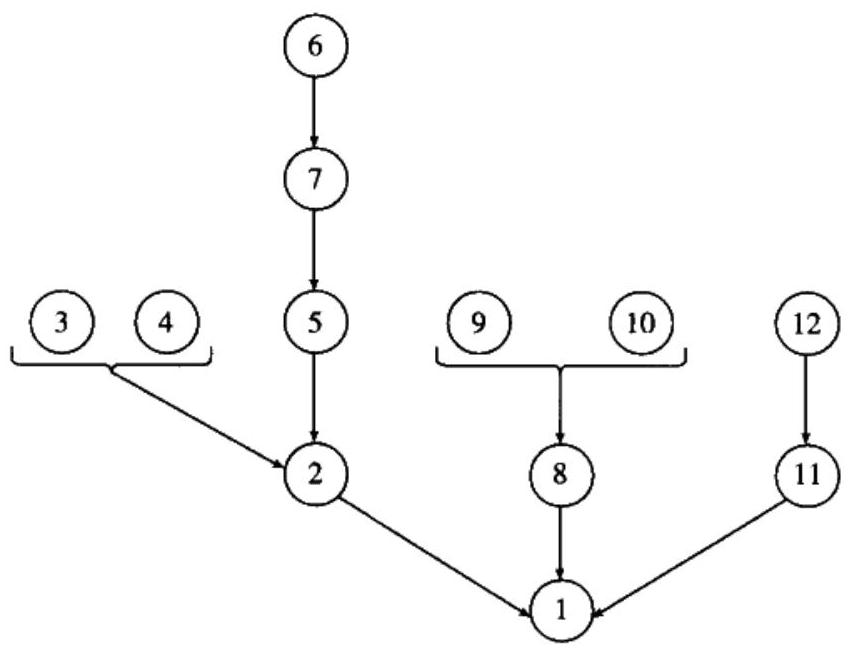
\includegraphics[width=\textwidth]{images/2025_05_15_6a28331d5e7c993ad07ag-076.jpg}
\end{center}

日常生活中的论证经常达不到这样的水准。它们可能包含着作用不清楚的陈述;论证中陈述与陈述之间的连接可能相互纠缠或被错述;甚至在论证者的头脑中论证的流程可能本来就是混乱的。由图示支持的\textbf{逻辑分析}可以暴露这些不足。通过使一个推理过程的结构暴露出来,我们能看到推理过程是如何展开的,推理的长处与缺陷是什么。逻辑学的一个特殊领域就是对实际论证的评估,成功的评估需要对所分析的论证有一个清楚的把握。

\chaptersummary{

  通过图示法展现复杂论证的逻辑结构,我们可以辨识出前提与结论间的关系,\\
  分析论证中的重复命题、浓缩前提,揭示推理的优缺点,\\
  从而更准确地评估复杂论证的有效性和可靠性。

} 